\documentclass[11pt]{article}

\usepackage{fontspec}
\usepackage[margin=1in]{geometry}
\usepackage{amsmath}
\usepackage{array}
\usepackage{booktabs}
\usepackage{xcolor}
\usepackage{listings}
\usepackage{needspace}
\usepackage{tikz}
\usetikzlibrary{arrows.meta,positioning}
\usepackage[hidelinks]{hyperref}

\lstdefinelanguage{Rust}{
  morekeywords={
    as,async,await,break,const,continue,crate,else,enum,extern,false,fn,for,if,impl,in,let,loop,match,mod,move,mut,pub,ref,return,self,Self,static,struct,super,trait,true,type,unsafe,use,where,while,
    Some,None,Option,Either,Left,Right,Pubkey,Signature,Ctx8,u8,u16,u32,u256,bool
  },
  sensitive=true,
  morecomment=[l]{//},
  morestring=[b]"
}

\lstset{
  basicstyle=\ttfamily\footnotesize,
  breaklines=true,
  breakatwhitespace=true,
  columns=fullflexible,
  frame=single,
  framerule=0.25pt,
  rulecolor=\color{black!55},
  framesep=6pt,
  xleftmargin=1.4em,
  xrightmargin=1.4em,
  aboveskip=0.75\baselineskip,
  belowskip=0.75\baselineskip,
  keepspaces=true,
  keywordstyle=\color{blue!65!black}\bfseries,
  commentstyle=\color{green!45!black},
  stringstyle=\color{orange!60!black},
  emph={assert},
  emphstyle=\color{red!65!black}\bfseries,
  language=Rust,
  showstringspaces=false
}

\title{Programmable Signatures with Simplicity}
\date{\today}

\begin{document}

\maketitle

\begin{abstract}
We propose a way for multisig participants to attach rules for spending their signatures.
For example, Alice can give a signature to spend a multisig with the condition that she receives 0.1 Bitcoin.
\end{abstract}

\section{Introduction}

With the introduction of Simplicity and Liquid \cite{simplicity,liquid}, we are now capable of transaction introspection
in much greater detail in comparison to regular Bitcoin Script \cite{bitcoin-whitepaper,bitcoin-dev-transactions}.

Multisigs are one of the most common logical structures in the Bitcoin ecosystem.
The most trivial one is the \texttt{OP\_CHECKMULTISIG} opcode \cite{bip11}.
Over time, different algorithms and standards appeared, such as deterministic pay-to-script-hash multi-signature addresses through public key sorting \cite{bip67}
and the general Taproot script validation rules in BIP 342 \cite{bip342}.
They allowed the ecosystem to customize how multiple users can spend a single UTXO.

Initiatives like FROST \cite{frost} optimize the amount of fees, which is out of scope for this paper.

Our goal is to provide even greater customization on top of Simplicity \cite{simplicity}.
The user can not only agree on spending the UTXO, but can also attach policies, such as pay-to-use checks, whitelist checks, compliance checks, and similar rules, to the spending signature.

\section{Building a Multisig Based on Simplicity}

\subsection{Message Construction}

The most sensitive part is the message that is signed by every participant.

In the basic version of the multisig \cite{native-multisig-multisig}, the message that is verified by users includes:

\begin{enumerate}
\item \texttt{jet::input\_hash(0..=i)} \cite{simplicity-input-hash}, where $i$ is the last multisig input;
\item \texttt{jet::output\_hash(0..=j)} \cite{simplicity-output-hash}, where $j$ is the last desired output;
\item policies that must be validated before allowing the use of the signature.
\end{enumerate}

Important note: in this model, not the whole transaction is signed.
Therefore, when a participant creates the message, the participant must ensure that, for example, when 1 LBTC is spent, all outputs that should be constrained are in the range $0..=j$.

As a result, the base message is:

\begin{equation}
\mathrm{base\_message}
  =
\mathrm{SHA256}(
  \mathrm{input\_hashes}
  \,\|\,
  \mathrm{output\_hashes}
).
\end{equation}

Every participant signs a message that also contains the executable leaf hash, which represents the set of policies:

\begin{equation}
\mathrm{participant\_message}
  =
\mathrm{SHA256}(
  \mathrm{vote\_executable\_leaf\_hash}
  \,\|\,
  \mathrm{base\_message}
).
\end{equation}

\subsection{Programmable Signature}

Below is a diagram of the Taproot tree, which generally represents a Taproot output that includes Simplicity with TapData included \cite{bip341,simplicity-state}.

\begin{figure}[ht]
  \centering
  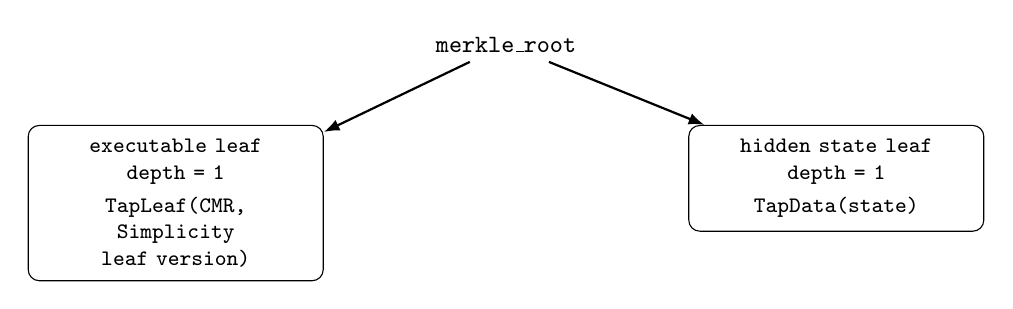
\begin{tikzpicture}[
    node distance=0.8cm and 1.3cm,
    root/.style={font=\ttfamily\small},
    box/.style={draw, rounded corners, align=center, font=\ttfamily\footnotesize,
      inner sep=5pt, text width=0.28\linewidth},
    arrow/.style={-{Latex[length=2mm]}, thick}
  ]
    \node[root] (root) {merkle\_root};
    \node[box, below left=of root] (exec) {
      executable leaf\\
      depth = 1\\[0.3em]
      TapLeaf(CMR,\\
      Simplicity leaf version)
    };
    \node[box, below right=of root] (state) {
      hidden state leaf\\
      depth = 1\\[0.3em]
      TapData(state)
    };

    \draw[arrow] (root) -- (exec);
    \draw[arrow] (root) -- (state);
  \end{tikzpicture}
  \caption{Vote Taproot tree with executable Simplicity leaf and hidden TapData state.}
\end{figure}

The hidden state leaf commits to the participant signature as follows:

\begin{equation}
\begin{aligned}
\mathrm{TapData(state)}
  = \mathrm{SHA256}(&
    \mathrm{SHA256}(\texttt{"TapData"}) \,\|\, \\
  &
    \mathrm{SHA256}(\texttt{"TapData"}) \,\|\, \\
  &
    \mathrm{SHA256}(\mathrm{participant\_signature})
  ).
\end{aligned}
\end{equation}

The executable leaf is the left part of the tree.
Simplicity's Taproot integration is described in the Simplicity Taproot work \cite{simplicity-taproot-universal-sighashes}.

This part contains all checks that Simplicity can perform, for example checking that one of the outputs sends Alice 0.1 BTC.

The implementation of the vote contract is in \texttt{vote.simf} \cite{native-multisig-vote}.

The right branch contains the signature part.
This part is needed by the multisig covenant to verify that the correct ``vote'' was included \cite{native-multisig-multisig}.

Because of the UTXO nature of Liquid, every vote would contain either a dust amount of LBTC or a throwaway token.
The exact asset or the way the vote is created is out of scope of this paper.

\section{Security Considerations}

\subsection{Threshold Checks}

The provided reference implementation of the multisig \cite{native-multisig-multisig} includes the basic n-of-3 check.
This means that three users can gather together and agree on the desired threshold.

If a bigger number of participants is expected, a contract modification is required due to compiler constraints.
At the time of writing this paper, SimplicityHL does not allow parameterizing the size of the array.

\Needspace{7\baselineskip}
The sanity checks of the threshold parameter are as follows:

\begin{lstlisting}
let threshold: u32 = param::THRESHOLD;
// Sanity checks to ensure that the multisig is spendable.
assert!(jet::le_32(1, threshold));
assert!(jet::le_32(threshold, 3));
\end{lstlisting}

\Needspace{12\baselineskip}
and:

\begin{lstlisting}
// Verification is done in the following order.
// Starting after the multisig inputs, if the signature for input i is None, skip it.
// Otherwise, calculate the expected vote script hash and check that it matches.
// Then check the signature against participants[i].
// This action is performed for all participants.
// Finally, check that the number of non-None signatures is greater than or equal to the threshold.
let (valid_votes, next_vote_input_index): (u32, u32) =
  count_votes(participants, votes, multisig_input_count, base_message);
assert!(jet::le_32(threshold, valid_votes));
\end{lstlisting}

With the last one, we iterate over provided user inputs.
It means that to spend the multisig input, it should have, for example, at least two votes if the threshold is two.

This constraint is related to the following check:

\begin{lstlisting}
// We need to ensure that during spending we have enough votes.
let (carry, minimum_inputs_num): (bool, u32) =
  jet::add_32(threshold, multisig_input_count);
ensure_zero_bit(carry);
assert!(jet::le_32(minimum_inputs_num, jet::num_inputs()));
\end{lstlisting}

This checks that the transaction has enough inputs to actually spend the transaction.
The logic is that, for example, to spend a 2-of-3 multisig, you need at least three inputs: one for the multisig and two for the vote covenants.

\subsection{Multisig Input and Output Windows}

Every multisig input is signed.

\begin{lstlisting}
// For every vote entry, verify the presence of the on-chain commitment
// and the correctness of the signed message.
fn count_vote_entry(
  entry: (Pubkey, Option<(Signature, u256)>),
  acc: (u32, u32, u256)
) -> (u32, u32, u256) {
  let (participant, maybe_vote): (Pubkey, Option<(Signature, u256)>) = entry;
  let (valid_votes, next_vote_input_index, base_message): (u32, u32, u256) = acc;

  let (valid_votes, next_vote_input_index): (u32, u32) = match maybe_vote {
    Some(vote: (Signature, u256)) => {
      let (participant_signature, vote_executable_leaf_hash): (Signature, u256) = vote;

      verify_vote_input(next_vote_input_index, vote_executable_leaf_hash, participant_signature);
      checksig(participant, participant_signature, vote_executable_leaf_hash, base_message);

      (increment_checked(valid_votes), increment_checked(next_vote_input_index))
    }
    None => (valid_votes, next_vote_input_index),
  };

  (valid_votes, next_vote_input_index, base_message)
}
\end{lstlisting}

In the covenant, until we reach the last non-multisig input, we collect the signatures:

\begin{lstlisting}
// Continue iterating over the inputs until the script hash no longer matches.
// This also enforces that multisig inputs start at index 0.
fn add_multisig_input_hash(acc: (Ctx8, u32), current_script_hash: u256, index: u8)
  -> Either<(Ctx8, u32), (Ctx8, u32)> {
  let (ctx, multisig_input_count): (Ctx8, u32) = acc;

  let index: u32 = jet::left_pad_low_8_32(index);
  let input_script_hash: Option<u256> = jet::input_script_hash(index);

  match input_script_hash {
    Some(input_script_hash: u256) => {
      match jet::eq_256(input_script_hash, current_script_hash) {
        true => {
          let next_ctx: Ctx8 =
            jet::sha_256_ctx_8_add_32(ctx, unwrap(jet::input_hash(index)));
          let next_multisig_input_count: u32 = increment_checked(multisig_input_count);
          Right((next_ctx, next_multisig_input_count))
        },
        false => Left((ctx, multisig_input_count)),
      }
    },
    None => Left((ctx, multisig_input_count)),
  }
}
\end{lstlisting}

The covenant verifies that if a multisig input is present, it is spent in the window from zero up to the last multisig input.
The covenant also checks that the current multisig input is included in the signed base message:

\begin{lstlisting}
let (base_message, multisig_input_count): (u256, u32) =
  base_message_and_input_count(witness::TOTAL_PROPOSED_OUTPUTS);
// Another sanity check: enforce that multisig covenant inputs start at index 0.
// This fails if the UTXO at index 0 is not a multisig.
assert!(jet::le_32(1, multisig_input_count));
// Ensure that the current multisig input is included in the signed base message.
assert!(jet::lt_32(jet::current_index(), multisig_input_count));
\end{lstlisting}

The second part that is included in the base message is the outputs.
During construction of the base message, they are included in the base message:

\begin{lstlisting}
// Build the base message that participants sign.
//
// The message signed by each participant includes all multisig inputs,
// i.e. jet::input_hash(i).
//
// It also includes outputs proposed by the participant,
// i.e. jet::output_hash(i).
fn base_message_and_input_count(total_proposed_outputs: u16) -> (u256, u32) {
  let ctx: Ctx8 = jet::sha_256_ctx_8_init();
  let input_result =
    for_while::<add_multisig_input_hash>((ctx, 0), jet::current_script_hash());

  let (ctx, multisig_input_count): (Ctx8, u32) = unwrap_left(input_result);
  let output_result = for_while::<add_proposed_output_hash>(ctx, total_proposed_outputs);

  let ctx: Ctx8 = unwrap_left(output_result);

  (jet::sha_256_ctx_8_finalize(ctx), multisig_input_count)
}
\end{lstlisting}

As shown above, in the final signature check we also append the \texttt{vote\_executable\_leaf\_hash}.
This leads to the last check: vote execution checks.

To check that the vote was included in the transaction, the multisig needs to check that an input with the desired policies is included.

\begin{lstlisting}
// This function verifies that the proved signature is committed on-chain
// through the intended vote.simf program.
// The intended vote.simf program is the one signed by the participant.
fn verify_vote_input(
  input_index: u32,
  vote_executable_leaf_hash: u256,
  participant_signature: Signature
) {
  let state_hash_ctx1: Ctx8 = jet::sha_256_ctx_8_init();
  let state_hash_ctx2: Ctx8 =
    jet::sha_256_ctx_8_add_64(state_hash_ctx1, Signature::into(participant_signature));
  let state_hash: u256 = jet::sha_256_ctx_8_finalize(state_hash_ctx2);

  let tap_leaf: u256 = vote_executable_leaf_hash;
  let state_ctx1: Ctx8 = jet::tapdata_init();
  let state_ctx2: Ctx8 = jet::sha_256_ctx_8_add_32(state_ctx1, state_hash);
  let state_leaf: u256 = jet::sha_256_ctx_8_finalize(state_ctx2);
  let tap_node: u256 = jet::build_tapbranch(tap_leaf, state_leaf);

  let bip0341_key: u256 =
    0x50929b74c1a04954b78b4b6035e97a5e078a5a0f28ec96d547bfee9ace803ac0;
  let tweaked_key: u256 = jet::build_taptweak(bip0341_key, tap_node);

  let hash_ctx1: Ctx8 = jet::sha_256_ctx_8_init();
  let hash_ctx2: Ctx8 = jet::sha_256_ctx_8_add_2(hash_ctx1, 0x5120);
  let hash_ctx3: Ctx8 = jet::sha_256_ctx_8_add_32(hash_ctx2, tweaked_key);
  let expected_vote_script_hash: u256 = jet::sha_256_ctx_8_finalize(hash_ctx3);

  assert!(jet::eq_256(
    unwrap(jet::input_script_hash(input_index)),
    expected_vote_script_hash
  ));
}
\end{lstlisting}

To do that, we reconstruct the Merkle tree and do the last assert:

\begin{lstlisting}
assert!(jet::eq_256(
  unwrap(jet::input_script_hash(input_index)),
  expected_vote_script_hash
));
\end{lstlisting}

This makes clear why the expected vote script hash is included in the message that is signed by the participant and how the multisig enforces a programmable check.
If the policies are changed, the signature verification fails.
Also, by Bitcoin consensus rules, when an input is included in the transaction that is being spent, the proper witness should be provided.

\subsection{Uncounted Vote Inputs}

There is a caveat on how uncounted votes can be spent; see \texttt{vote.simf} for more details \cite{native-multisig-vote}.

In a nutshell, during a 1-of-3 multisig execution, all three votes can be provided, but only one of them is needed to be checked.
From the multisig perspective, this is fine because the threshold is met.
However, the value that the vote holds can be moved to any address if it is not constrained by the message that is signed.
Dealing with this issue is out of scope of this paper.
Enough information and a mitigation solution are mentioned in the code.

\section{Coordination}

Another part that we touched on preliminarily is coordination between participants.
Coordination can be done in two ways: off chain and on chain.

Off-chain coordination is obvious.
Participants use a shared communication channel to exchange the data.
This allows them to spend any transaction regardless of its weight.

On the other hand, the reference implementation also supports on-chain coordination \cite{native-multisig-onchain-encoder}.
It uses \texttt{OP\_RETURN} outputs.

During multisig creation, the multisig itself is always represented by the P2TR address, which is static because the Merkle tree only depends on the multisig configuration.
It does not allow changing the participant or threshold dynamically.

Every participant can attach, via \texttt{OP\_RETURN}s, their descriptors with which they will publish votes.
Alongside votes, they provide enough information in \texttt{OP\_RETURN}s for other participants to create the same votes.

For example, the regtest scenarios include a 2-of-3 spend with one multisig input and two vote inputs, and another spend with two multisig inputs, two vote inputs, and three proposed outputs \cite{native-multisig-regtest}.
Those examples demonstrate the intended transaction shape: multisig inputs first, vote inputs after the multisig input window, and proposed outputs starting from output index zero.

\section{Bitcoin Compatibility}

Even though the multisig is based on Simplicity, there is ongoing work to add Simplicity to Bitcoin Inquisition \cite{bitcoin-inquisition-binana-simplicity,bitcoin-inquisition-simplicity-impl}.

All core jets that were used in the current multisig will be present in the Bitcoin version as well.
Therefore, this solution is Bitcoin-compatible if Simplicity is ever added to Bitcoin itself.

\section{Formal Verification}

The work on formal verification of the contract is ongoing.
Details of it will be mentioned when it is done.

\bibliographystyle{unsrt}
\bibliography{references}

\end{document}
